\documentclass[12pt,letterpaper]{article}
\usepackage{graphicx,textcomp}
\usepackage{natbib}
\usepackage{setspace}
\usepackage{fullpage}
\usepackage{color}
\usepackage[reqno]{amsmath}
\usepackage{amsthm}
\usepackage{fancyvrb}
\usepackage{amssymb,enumerate}
\usepackage[all]{xy}
\usepackage{endnotes}
\usepackage{lscape}
\newtheorem{com}{Comment}
\usepackage{float}
\usepackage{hyperref}
\newtheorem{lem} {Lemma}
\newtheorem{prop}{Proposition}
\newtheorem{thm}{Theorem}
\newtheorem{defn}{Definition}
\newtheorem{cor}{Corollary}
\newtheorem{obs}{Observation}
\usepackage[compact]{titlesec}
\usepackage{dcolumn}
\usepackage{tikz}
\usetikzlibrary{arrows}
\usepackage{multirow}
\usepackage{xcolor}
\newcolumntype{.}{D{.}{.}{-1}}
\newcolumntype{d}[1]{D{.}{.}{#1}}
\definecolor{light-gray}{gray}{0.65}
\usepackage{url}
\usepackage{listings}
\usepackage{color}

\definecolor{codegreen}{rgb}{0,0.6,0}
\definecolor{codegray}{rgb}{0.5,0.5,0.5}
\definecolor{codepurple}{rgb}{0.58,0,0.82}
\definecolor{backcolour}{rgb}{0.95,0.95,0.92}

\lstdefinestyle{mystyle}{
	backgroundcolor=\color{backcolour},   
	commentstyle=\color{codegreen},
	keywordstyle=\color{magenta},
	numberstyle=\tiny\color{codegray},
	stringstyle=\color{codepurple},
	basicstyle=\footnotesize,
	breakatwhitespace=false,         
	breaklines=true,                 
	captionpos=b,                    
	keepspaces=true,                 
	numbers=left,                    
	numbersep=5pt,                  
	showspaces=false,                
	showstringspaces=false,
	showtabs=false,                  
	tabsize=2
}
\lstset{style=mystyle}
\newcommand{\Sref}[1]{Section~\ref{#1}}
\newtheorem{hyp}{Hypothesis}

\title{Problem Set 3}
\date{Due: November 11, 2024}
\author{Applied Stats/Quant Methods 1}


\begin{document}
	\maketitle
	\section*{Instructions}
	\begin{itemize}
		\item Please show your work! You may lose points by simply writing in the answer. If the problem requires you to execute commands in \texttt{R}, please include the code you used to get your answers. Please also include the \texttt{.R} file that contains your code. If you are not sure if work needs to be shown for a particular problem, please ask.
	\item Your homework should be submitted electronically on GitHub.
	\item This problem set is due before 23:59 on Sunday November 11, 2024. No late assignments will be accepted.

	\end{itemize}

		\vspace{.25cm}
	
\noindent In this problem set, you will run several regressions and create an add variable plot (see the lecture slides) in \texttt{R} using the \texttt{incumbents\_subset.csv} dataset. Include all of your code.

	\vspace{.5cm}
\section*{Question 1}
\vspace{.25cm}
\noindent We are interested in knowing how the difference in campaign spending between incumbent and challenger affects the incumbent's vote share. 
	\begin{enumerate}
		\item 
		Run a regression where the outcome variable is \texttt{voteshare} and the explanatory variable is \texttt{difflog}.\\ 
		
		\noindent Using the function lm() in R, I name my regression 	q\_1\_regression and use the dataset I named inc.sub.
		\begin{verbatim}
		> q_1_regression <- lm(formula = voteshare ~ difflog, data = inc.sub)
		> summary(q_1_regression)
		
		Call:
		lm(formula = voteshare ~ difflog, data = inc.sub)
		
		Residuals:
		Min       1Q   Median       3Q      Max 
		-0.26832 -0.05345 -0.00377  0.04780  0.32749 
		
		Coefficients:
		Estimate Std. Error t value Pr(>|t|)    
		(Intercept) 0.579031   0.002251  257.19   <2e-16 ***
		difflog     0.041666   0.000968   43.04   <2e-16 ***
		---
		Signif. codes:  0 ‘***’ 0.001 ‘**’ 0.01 ‘*’ 0.05 ‘.’ 0.1 ‘ ’ 1
		
		Residual standard error: 0.07867 on 3191 degrees of freedom
		Multiple R-squared:  0.3673,	Adjusted R-squared:  0.3671 
		F-statistic:  1853 on 1 and 3191 DF,  p-value: < 2.2e-16
	\end{verbatim}
	When difflog is zero (meaning equal campaign spending), the model predicts that the incumbent’s vote share would be approximately 57.9\%\ (intercept).
	
	For every one-unit increase in difflog (indicating the incumbent spends more than the challenger), the incumbent’s vote share increases by about 4.17 percentage points (slope - difflog coefficient). (positive link between higher relative spending by the incumbent and an increase in their vote share)
	
	The effect of difflog on voteshare is statistically significant, with a very low p-value (p less than 0.001), indicating that this result is unlikely due to chance.
	
	The R-squared of 0.3673 suggests that about 36.7\%\ of the variability in vote share is explained by campaign spending differences, with the remaining variation due to other factors.
	
	I am going to repeat this general process for Question 2 and 3.
		\item Make a scatterplot of the two variables and add the regression line. 	\\
		
		First I create a scatterplot using 
		\begin{verbatim}
		> plot(inc.sub$difflog, inc.sub$voteshare)
	\end{verbatim}
	Then (so the line is visible on top of all datapoints) I create a red line on top of the graph using
	\begin{verbatim}
		abline(lm(voteshare ~ difflog, data = inc.sub), col="red")
	\end{verbatim}
	This gives me the following graph: \\
 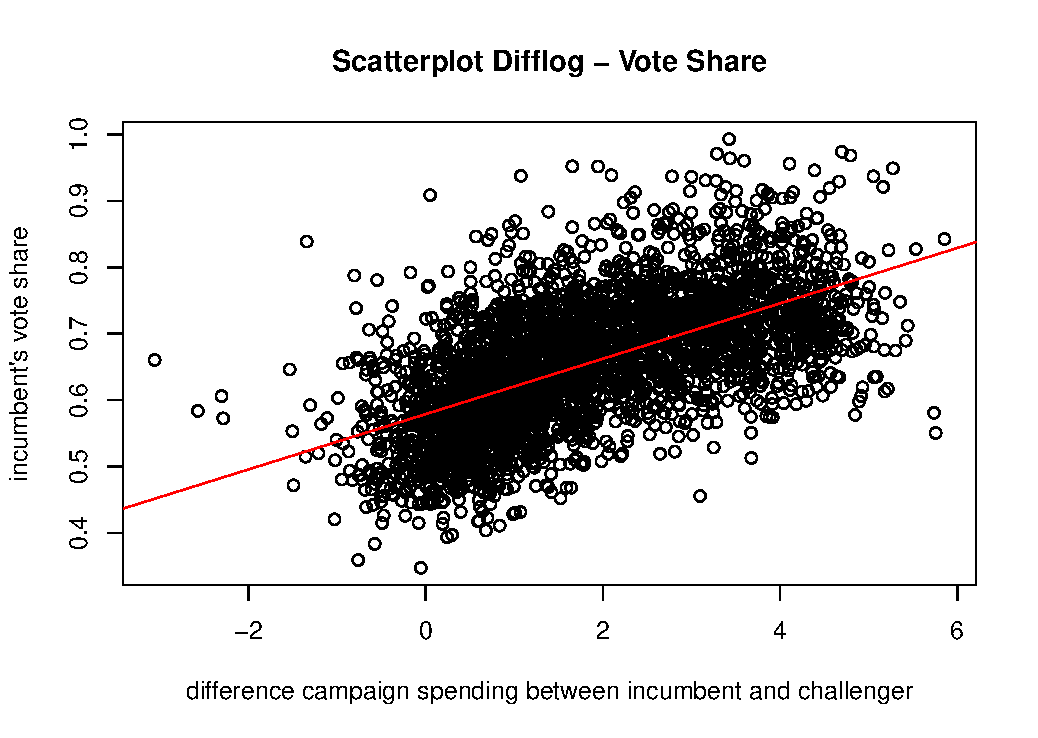
\includegraphics[width=\textwidth,height=\textheight,keepaspectratio]{Q_1_Plot}
 I am going to repeat this same process for Question 2 and Question 3.
	
		\item Save the residuals of the model in a separate object.	\\
		
		I named the object to save my residuals in q\_1\_residuals and created it in the following way. I am going to repeat this pattern in Question 2 as well.
		\begin{verbatim}
		> q_1_residuals <- q_1_regression$residuals
	\end{verbatim}
		\item Write the prediction equation. \\
		
		Using the numbers calculated with
			\begin{verbatim}
			> q_1_regression <- lm(formula = voteshare ~ difflog, data = inc.sub)
		\end{verbatim}
		Specifically relevant to me are the Intercept Coefficient Estimate and the variable (difflog) Coefficient Estimate.
		
		So in this case I get \\
		Y = 0.579031 + 0.041666 * X \\
		Or in our specific case: \\
		voteshare = 0.579031 + 0.041666 * difflog \\
		Incumbent's Vote Share = 0.579031 + 0.041666 * difference in campaign spending between incumbent and challenger
	\end{enumerate}
	
\newpage

\section*{Question 2}
\noindent We are interested in knowing how the difference between incumbent and challenger's spending and the vote share of the presidential candidate of the incumbent's party are related.	\vspace{.25cm}
	\begin{enumerate}
		\item Run a regression where the outcome variable is \texttt{presvote} and the explanatory variable is \texttt{difflog}.	\\
		\begin{verbatim}
			> q_2_regression<-lm(formula = presvote ~ difflog, data = inc.sub)
			> summary(q_2_regression)
			
			Call:
			lm(formula = presvote ~ difflog, data = inc.sub)
			
			Residuals:
			Min       1Q   Median       3Q      Max 
			-0.32196 -0.07407 -0.00102  0.07151  0.42743 
			
			Coefficients:
			Estimate Std. Error t value Pr(>|t|)    
			(Intercept) 0.507583   0.003161  160.60   <2e-16 ***
			difflog     0.023837   0.001359   17.54   <2e-16 ***
			---
			Signif. codes:  
			0 ‘***’ 0.001 ‘**’ 0.01 ‘*’ 0.05 ‘.’ 0.1 ‘ ’ 1
			
			Residual standard error: 0.1104 on 3191 degrees of freedom
			Multiple R-squared:  0.08795,	Adjusted R-squared:  0.08767 
			F-statistic: 307.7 on 1 and 3191 DF,  p-value: < 2.2e-16
		\end{verbatim}
		When difflog is zero (meaning equal campaign spending), the model predicts that a presidential vote share of approximately 50.8\%\ (intercept).
		
		For every one-unit increase in difflog (indicating the incumbent spends more than the challenger), the presidential vote share increases by about 2.38 percentage points (slope - difflog coefficient). (positive link between higher relative spending by the incumbent and increase in their presidential candidate's success)
		
		The effect of difflog on presvote is statistically significant (p less than 0.001).
		
		The R-squared of 0.088 suggests that about 8.8\%\ of the variability in the presidential vote share is explained by campaign spending differences, with the remaining variation due to other factors. (other factors beyond campaign spending differences play a substantial role in determining the presidential candidate's vote share)
		
		\item Make a scatterplot of the two variables and add the regression line.  \\
		\begin{verbatim}
> plot(inc.sub$difflog, inc.sub$presvote, 
+      xlab = "difference between incumbent's and challenger's spending",
+      ylab = "vote share of the presidential candidate of the incumbent's party",
+      main = "Scatterplot Difflog - Presvote")
> abline(lm(presvote ~ difflog, data = inc.sub), col="red")
	\end{verbatim}
	 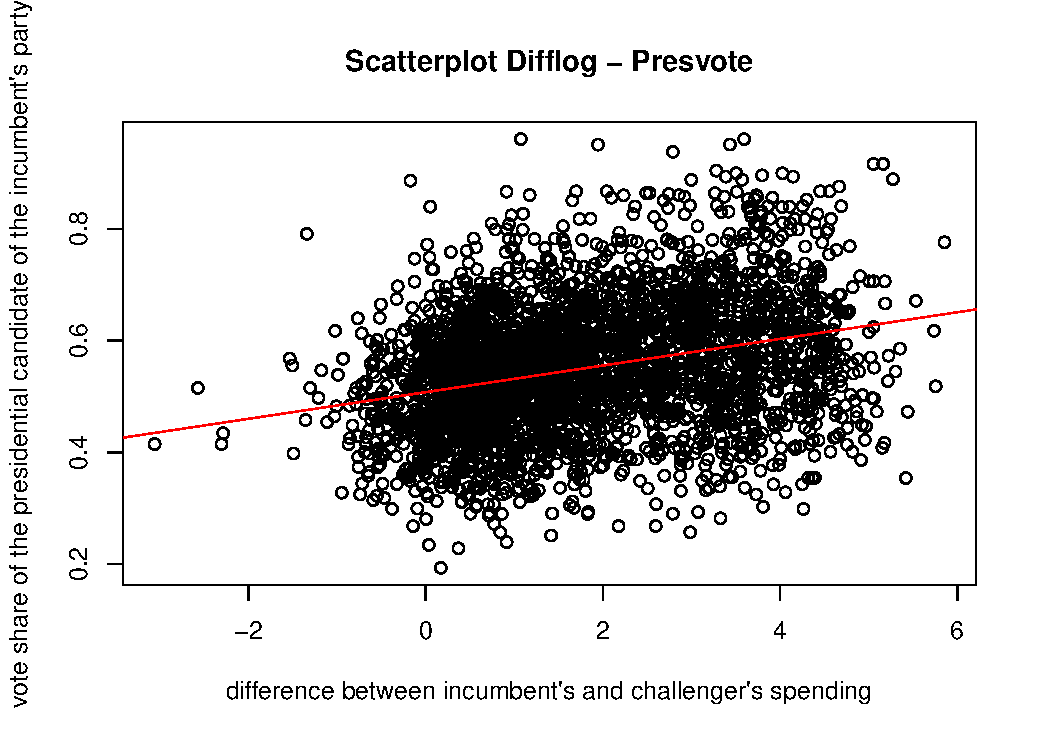
\includegraphics[width=\textwidth,height=\textheight,keepaspectratio]{Q_2_Plot}
		\item Save the residuals of the model in a separate object.	\\
		\begin{verbatim}
		q_2_residuals <- lm(formula = presvote ~ difflog, data = inc.sub)$residuals
	\end{verbatim}
		\item Write the prediction equation.
		Using the numbers calculated with
		\begin{verbatim}
			q_2_regression<-lm(formula = presvote ~ difflog, data = inc.sub)
		\end{verbatim}
		I get \\
		Y = 0.507583 + 0.023837 * X \\
		Or in our specific case: \\
		presvote = 0.507583 + 0.023837 * difflog \\
		vote share of the presidential candidate of the incumbent's party = 0.507583 + 0.023837 * difference in campaign spending between incumbent and challenger
	\end{enumerate}
	
	\newpage	
\section*{Question 3}

\noindent We are interested in knowing how the vote share of the presidential candidate of the incumbent's party is associated with the incumbent's electoral success.
	\vspace{.25cm}
	\begin{enumerate}
		\item Run a regression where the outcome variable is \texttt{voteshare} and the explanatory variable is \texttt{presvote}. 
		\begin{verbatim}
			> q_3_regression<-lm(formula = voteshare ~ presvote, data = inc.sub)
			> summary(q_3_regression)
			
			Call:
			lm(formula = voteshare ~ presvote, data = inc.sub)
			
			Residuals:
			Min       1Q   Median       3Q      Max 
			-0.27330 -0.05888  0.00394  0.06148  0.41365 
			
			Coefficients:
			Estimate Std. Error t value Pr(>|t|)    
			(Intercept) 0.441330   0.007599   58.08   <2e-16 ***
			presvote    0.388018   0.013493   28.76   <2e-16 ***
			---
			Signif. codes:  
			0 ‘***’ 0.001 ‘**’ 0.01 ‘*’ 0.05 ‘.’ 0.1 ‘ ’ 1
			
			Residual standard error: 0.08815 on 3191 degrees of freedom
			Multiple R-squared:  0.2058,	Adjusted R-squared:  0.2056 
			F-statistic:   827 on 1 and 3191 DF,  p-value: < 2.2e-16
		\end{verbatim}

		When presvote is zero (purely hypothetically the presidential candidate of the incumbent’s party receives no votes), model predicts an incumbent vote share (voteshare) of about 44.1\%\. (This number is harder to interpret, might suggest strong base of support for the incumbent party, no matter the presidential candidate).
		
		For every one-unit increase in presvote (representing a 1\%\ increase in the presidential candidate’s vote share), the incumbent’s vote share increases by about 0.39\%\ (slope - presvote coefficient).
		
		The low p-value (p less than 0.001) for presvote shows this effect is statistically significant. 
		
		The R-squared of 0.206 suggests that about 20.6\%\ of the variability iincumbent’s vote share is explained by the presidential vote share.
		
		\item Make a scatterplot of the two variables and add the regression line. \\
		\begin{verbatim}
		> plot(inc.sub$presvote, inc.sub$voteshare,
		+      xlab = "vote share of the presidential candidate of the incumbent's party",
		+      ylab = "incumbent's electoral success",
		+      main = "Scatterplot Presvote - Voteshare")
		> abline(lm(voteshare ~ presvote, data = inc.sub), col="red")
			\end{verbatim} 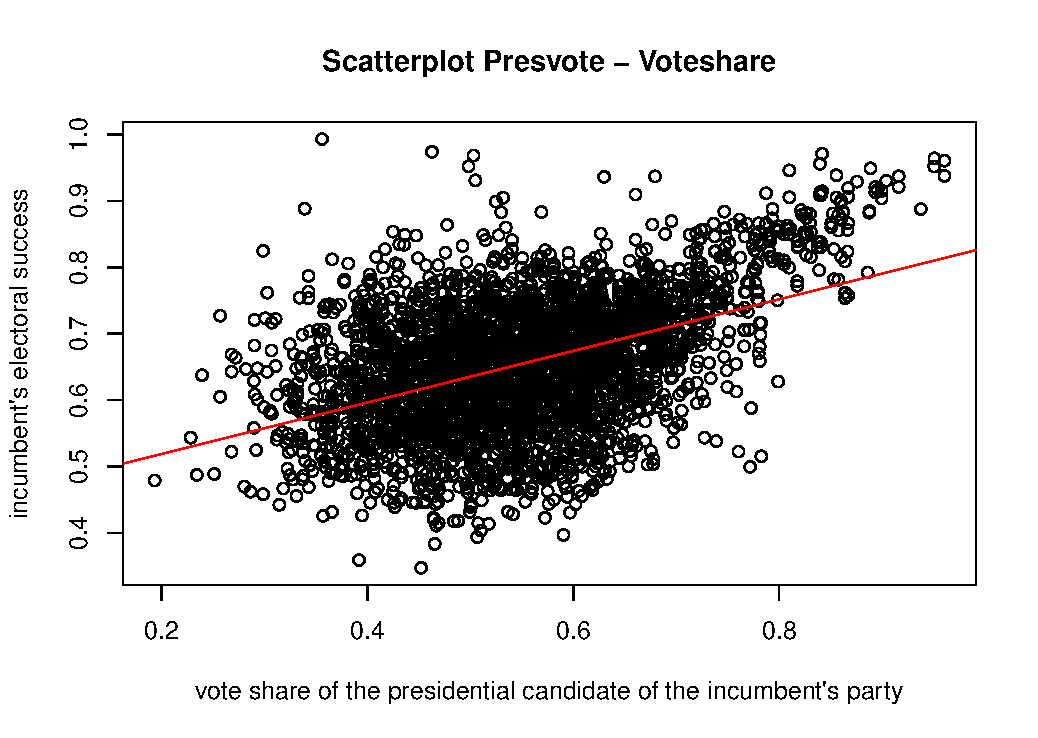
\includegraphics[width=\textwidth,height=\textheight,keepaspectratio]{Q_3_Plot}
		\item Write the prediction equation.\\
		
		Using the numbers calculated with
		\begin{verbatim}
			> q_3_regression<-lm(formula = voteshare ~ presvote, data = inc.sub)
		\end{verbatim}
		I get \\
		Y=0.441330 +0.388018 * X \\
		Or in our specific case: \\
		voteshare = 0.441330 + 0.388018 * presvote \\
		incumbent's electoral success = 0.441330 + 0.388018  * vote share of the presidential candidate of the incumbent's party
	
	\end{enumerate}
	

\newpage	
\section*{Question 4}
\noindent The residuals from part (a) tell us how much of the variation in \texttt{voteshare} is $not$ explained by the difference in spending between incumbent and challenger. The residuals in part (b) tell us how much of the variation in \texttt{presvote} is $not$ explained by the difference in spending between incumbent and challenger in the district.
	\begin{enumerate}
		\item Run a regression where the outcome variable is the residuals from Question 1 and the explanatory variable is the residuals from Question 2. \\
		
		q\_1\_residuals and q\_2\_residuals are the saved residuals from Question 1 and Question 2 respectively. Using these, I just run the regression in the same way as before, only this time I am not specifying the dataset as the variables that I created myself are not tied directly to the dataset inc.sub.
			\begin{verbatim}
		> q_4_regression<-lm(formula = q_1_residuals ~ q_2_residuals)
		> summary(q_4_regression)
		
		Call:
		lm(formula = q_1_residuals ~ q_2_residuals)
		
		Residuals:
		Min       1Q   Median       3Q      Max 
		-0.25928 -0.04737 -0.00121  0.04618  0.33126 
		
		Coefficients:
		Estimate Std. Error t value Pr(>|t|)    
		(Intercept)   -1.942e-18  1.299e-03    0.00        1    
		q_2_residuals  2.569e-01  1.176e-02   21.84   <2e-16 ***
		---
		Signif. codes:  
		0 ‘***’ 0.001 ‘**’ 0.01 ‘*’ 0.05 ‘.’ 0.1 ‘ ’ 1
		
		Residual standard error: 0.07338 on 3191 degrees of freedom
		Multiple R-squared:   0.13,	Adjusted R-squared:  0.1298 
		F-statistic:   477 on 1 and 3191 DF,  p-value: < 2.2e-16
	\end{verbatim}
	
	The intercept here is approximately zero (-1.942e-18) and statistically insignificant, which makes sense because the residuals should theoretically be centered around zero. 
	
	For each one-unit increase in q\_2\_residuals, q\_1\_residuals increases by approximately 0.257 units.
	
	The low p-value (p less than 0.001) for q\_2\_residuals indicates that this relationship is statistically significant.
	
	The R-squared value of 0.13 indicates that 13\% of the variance in q\_1\_residuals is explained by q\_2\_residuals, so much of the variability in q\_1\_residuals should be explained by other factors.
	
		\item Make a scatterplot of the two residuals and add the regression line. 	\\
		
		Using the exact same procedure as in the previous Questions, only this time using the values q\_1\_residuals and q\_2\_residuals I created and saved myself:
		\begin{verbatim}
		> plot(q_2_residuals, q_1_residuals,
		+      xlab = "variation presvote not explained by difference in spending",
		+      ylab = "variation voteshare not explained by difference in spending",
		+      main = "Scatterplot Residuals Q1 - Q2")
		> abline(lm(formula = q_2_residuals ~ q_1_residuals, data = inc.sub), col="red")
	\end{verbatim}
	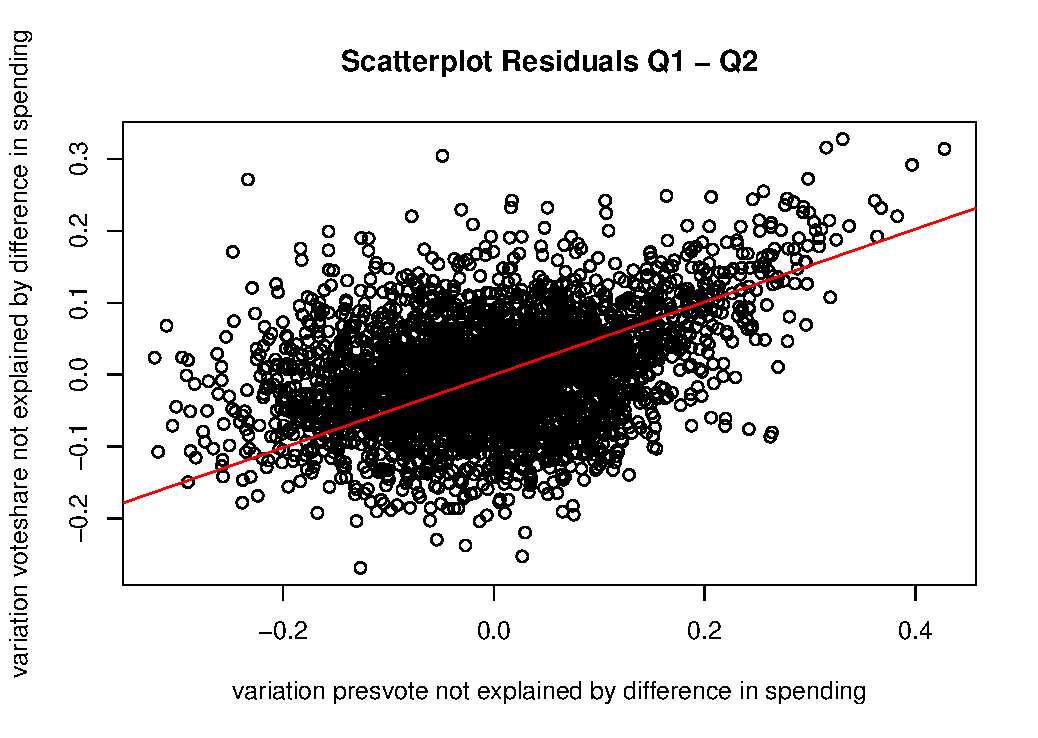
\includegraphics[width=\textwidth,height=\textheight,keepaspectratio]{Q_4_Plot}
		\item Write the prediction equation. \\
		
		Using the numbers calculated with
		\begin{verbatim}
			> q_4_regression<-lm(formula = q_1_residuals ~ q_2_residuals)
		\end{verbatim}
		I get: \\
		Y=-1.942e-18+2.569e-01 * X \\
		Or in our specific case: \\
		Q\_1\_residuals = -1.942e-18 + 2.569e-01 * Q\_2\_residuals \\
		amount of variation in voteshare not explained by the difference in spending between incumben and challenger = -1.942e-18 + 2.569e-01 * amount of variation in presvote not explained by the difference in spending between incumbent and challenger in the district \\
		The intercept is very close to 0 (almost negligible). 
	\end{enumerate}
	
	\newpage	

\section*{Question 5}
\noindent What if the incumbent's vote share is affected by both the president's popularity and the difference in spending between incumbent and challenger? 
	\begin{enumerate}
		\item Run a regression where the outcome variable is the incumbent's \texttt{voteshare} and the explanatory variables are \texttt{difflog} and \texttt{presvote}.	\\
		
		I essentially run the same regression lm() in R as before, only this time I connect the second explanatory variable to the first with a "+"
		\begin{verbatim}
		> q_5_regression<-lm(voteshare ~ difflog + presvote, data = inc.sub)
		> summary(q_5_regression)
		
		Call:
		lm(formula = voteshare ~ difflog + presvote, data = inc.sub)
		
		Residuals:
		Min       1Q   Median       3Q      Max 
		-0.25928 -0.04737 -0.00121  0.04618  0.33126 
		
		Coefficients:
		Estimate Std. Error t value Pr(>|t|)    
		(Intercept) 0.4486442  0.0063297   70.88   <2e-16 ***
		difflog     0.0355431  0.0009455   37.59   <2e-16 ***
		presvote    0.2568770  0.0117637   21.84   <2e-16 ***
		---
		Signif. codes:  
		0 ‘***’ 0.001 ‘**’ 0.01 ‘*’ 0.05 ‘.’ 0.1 ‘ ’ 1
		
		Residual standard error: 0.07339 on 3190 degrees of freedom
		Multiple R-squared:  0.4496,	Adjusted R-squared:  0.4493 
		F-statistic:  1303 on 2 and 3190 DF,  p-value: < 2.2e-16
	\end{verbatim}
	
	The intercept indicates that when both difflog (campaign spending difference) and presvote (presidential vote share) are zero, the incumbent’s vote share (voteshare) would be around 0.449, or 44.9\%., representing a baseline vote share for the party, without the influence of either campaign spending differences or the presidential candidate’s performance.
	
	For each unit increase in difflog, voteshare is expected to increase by around 0.0355 units, if prevote remains the same. 
	
	For each unit increase in presvote, voteshare is expected to increase by around 0.257 units, if difflog remains the same.
	
	Both difflog and presvote have p-values well below 0.001, showing statistically significant effects on voteshare. 
	
	The R-squared of 0.4496 means that 44.96\% of the variance in voteshare is explained by difflog and presvote. (means that the model captures a lot of variation in the incumbent’s vote share based on these two predictors)
	
		\item Write the prediction equation.	\\
		
		I get: \\
		Y=0.4486442 + 0.0355431 * X\_1 + 0.2568770 * X\_2\\
		Or in our specific case: \\
		voteshare = 0.4486442 + 0.0355431 * difflog + 0.2568770 * presvote\\
		incumbent's vote share =  0.4486442 + 0.0355431 * difference in spending between incumbent and challenger + 0.2568770 * president's popularity \\
		\item What is it in this output that is identical to the output in Question 4? Why do you think this is the case? \\
		
		The coefficient for q\_2\_residuals in q\_4\_regression (0.2569) is identical to the coefficient for presvote in q\_5\_regression (rounded 0.2569).
		
		This is because q\_4\_regression is regressing the residuals of voteshare ~ difflog on the residuals of presvote ~ difflog. This isolates the effect of presvote on voteshare while controlling for difflog. 
		
		In q\_5\_regression, both difflog and presvote are directly included in the model as explanatory variables, so the effect of presvote on voteshare in the presence of difflog is similarly isolated.
		
		This isolation also explains why the standard error and t-value for presvote in q\_5\_regression match the standard error and t-value for q\_2\_residuals in q\_4\_regression. Both sets of statistics reflect the same underlying relationship between voteshare and presvote while controlling for difflog.
		
		The residual summaries are also identical across models because both produce residuals based on the relationship between voteshare and the combination of difflog and presvote.
		
		Applying this explanation to the real meanings of the variables, both models isolate the influence of the incumbent’s party’s presidential success on the incumbent’s vote share, while controlling for the difference in campaign spending between incumbent and challenger.
		
		Tldr: coefficient, standard error and t-value for presvote and the residual summary statistics are identical in both outputs
		because, in both models, the effect of presvote on voteshare is isolated
		while controlling for difflog, either by regressing the residuals (q\_4\_regression) 
		or by including both variables in a multivariate model (q\_5\_regression).
	\end{enumerate}




\end{document}
